% ---
% school: "college"
% level: "8eme"
% section: null
% chapter: "التناظر المركزي"
% source: "Axiomaths"
% title: "مناظرة دائرة"
% country: "Tunisie"
% year: 2026
% professor: "Axiomaths"
% difficulty: "Facile"
% points: null
% tags: ["symetrie-centrale", "cercle", "tangente", "quadrillage"]
% ---
% Exercice 5/15 de la série 8ème « التناظر المركزي » (statement + \axsol + solution). Compiler avec XeLaTeX + axiomath.sty (+ axiomaths-logo.png).
\documentclass[12pt,a4paper]{article}
\usepackage[level=8b,color=15803D]{axiomath}
\usetikzlibrary{arrows.meta}
\newcommand{\cm}{\,\mathrm{cm}}
\axsetup{title={التناظر المركزي}, corrige}

\begin{document}

\begin{corr}[title={مناظرة دائرة}, stars=2, source={Axiomaths}]
$\mathcal{C}$ دائرة مركزها $I$ وشعاعها $2$ وحدات، $T$ نقطة منها، و $d$ المستقيم العمودي على $(IT)$ في $T$ ؛ $O$ نقطة معلومة.
\begin{center}
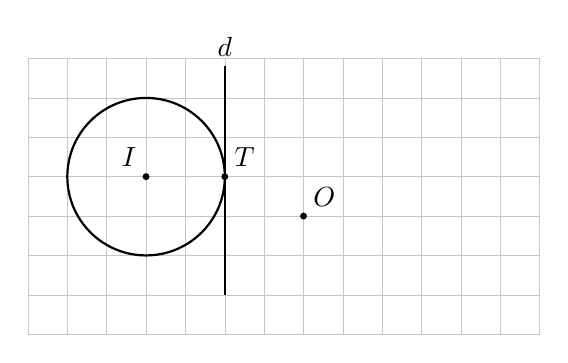
\begin{tikzpicture}[scale=0.5]
  \draw[gray!45,very thin] (0,0) grid (13,7);
  \draw[thick] (3,4) circle (2);
  \draw[thick] (5,1) -- (5,6.8) node[above] {$d$};
  \fill (3,4) circle (2.5pt) node[above left] {$I$};
  \fill (5,4) circle (2.5pt) node[above right] {$T$};
  \fill (7,3) circle (2.5pt) node[above right] {$O$};
\end{tikzpicture}
\end{center}
\begin{enumerate}
  \item ابنِ $I'$ مناظرة $I$ بالنسبة إلى $O$ ثم الدائرة $\mathcal{C}'$ مناظرة $\mathcal{C}$. ما هو شعاعها ؟
  \item ابنِ $T'$ مناظرة $T$ ثم المستقيم $d'$ مناظر $d$.
  \item بين أن $d'$ عمودي على $(I'T')$ في $T'$. ماذا تستنتج بالنسبة إلى $d'$ و $\mathcal{C}'$ ؟
\end{enumerate}
\axsol
\begin{enumerate}[itemsep=14pt]
  \item\leavevmode
  \begin{prop}[مناظرة دائرة]
  مناظرة الدائرة $\mathcal{C}(I\,;r)$ بالنسبة إلى $O$ هي الدائرة $\mathcal{C}'(I'\,;r)$ ، حيث $I'=S_O(I)$ : \ib{نفس الشعاع}.
  \end{prop}
  من $I$ إلى $O$ : 4 وحدات يمينا ووحدة إلى الأسفل ؛ نواصل بنفس الانتقال فنجد $I'$. شعاع $\mathcal{C}'$ هو $2$ وحدات.
  \item من $T$ إلى $O$ : وحدتان يمينا ووحدة إلى الأسفل ؛ نواصل فنجد $T'$. المستقيم $d$ يوازي مناظره : $d'$ هو المستقيم الموازي لـ $d$ والمار من $T'$.
  \begin{center}
  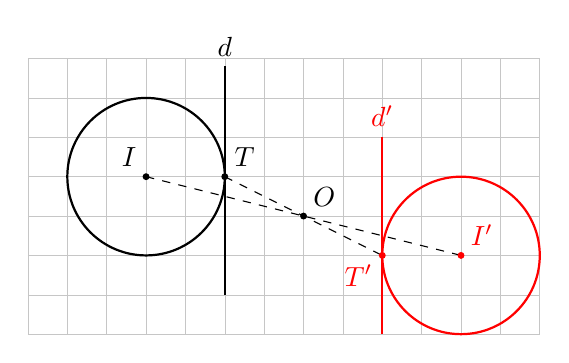
\begin{tikzpicture}[scale=0.5]
    \draw[gray!45,very thin] (0,0) grid (13,7);
    \draw[thick] (3,4) circle (2);
    \draw[thick] (5,1) -- (5,6.8) node[above] {$d$};
    \draw[thick,red] (11,2) circle (2);
    \draw[thick,red] (9,0) -- (9,5) node[above] {$d'$};
    \draw[dashed] (3,4)--(11,2);
    \draw[dashed] (5,4)--(9,2);
    \fill (3,4) circle (2.5pt) node[above left] {$I$};
    \fill (5,4) circle (2.5pt) node[above right] {$T$};
    \fill (7,3) circle (2.5pt) node[above right] {$O$};
    \fill[red] (11,2) circle (2.5pt) node[above right] {$I'$};
    \fill[red] (9,2) circle (2.5pt) node[below left] {$T'$};
  \end{tikzpicture}
  \end{center}
  \item $d\perp(IT)$ في $T$ ، والتناظر المركزي يحفظ قيس الزوايا ويحوّل $I$ إلى $I'$ و $T$ إلى $T'$ و $d$ إلى $d'$. إذن $d'\perp(I'T')$ في $T'$.
  بما أن $I'T'=IT=2$ فإن $T'\in\mathcal{C}'$ ، و $d'$ عمودي على الشعاع $[I'T']$ عند طرفه : $d'$ يقطع $\mathcal{C}'$ في نقطة وحيدة هي $T'$. \ib{$d'$ مماس لـ $\mathcal{C}'$ في $T'$}.
\end{enumerate}
\end{corr}

\end{document}
